\documentclass[10pt,ignorenonframetext,xcolor={dvipsnames, table}]{beamer}

%\usepackage{amssymb,amsmath}
\usepackage{textcomp}
\usepackage{ifxetex,ifluatex}
\usepackage{fixltx2e} % provides \textsubscript
\frenchspacing % single space after a period

\ifnum 0\ifxetex 1\fi\ifluatex 1\fi=0 % if pdftex
    %\usepackage{mathpazo}
    % \usepackage{lmodern}
  % \usepackage[sfdefault,light,condensed]{roboto}
  \usepackage{PTSansNarrow} 
  \usepackage[T1]{fontenc}
  \usepackage[utf8]{inputenc}
  % \usepackage{mathpazo}
\else % if luatex or xelatex
  \usepackage{fontspec}
  \usepackage{realscripts}
  \usepackage{unicode-math}
  \unimathsetup{math-style=TeX}

\fi

\usetheme{Madrid}


\setbeamertemplate{footline}[frame number]

\useinnertheme{rectangles}

\usefonttheme{structurebold}


\setbeamertemplate{bibliography item}{}
\setbeamertemplate{caption}[numbered]
\setbeamertemplate{frametitle continuation}[from second]
\setbeamertemplate{blocks}[rounded][shadow=false]
\resetcounteronoverlays{exx}
\beamertemplatenavigationsymbolsempty
\setbeamercovered{transparent}

\setbeamercolor{title}{bg=RoyalBlue}
\setbeamercolor{frametitle}{fg=White,bg=RoyalBlue}
\setbeamercolor{section in head/foot}{bg=RoyalBlue}
\setbeamercolor{author in head/foot}{bg=RoyalBlue}
\setbeamercolor{title in head/foot}{bg=RoyalBlue}
\setbeamercolor{date in head/foot}{bg=RoyalBlue}

\setbeamercolor{block title}{bg=RoyalBlue}
\setbeamercolor{block body}{bg=RoyalBlue!10}
\setbeamercolor*{caption name}{fg=RoyalBlue}
\setbeamercolor*{item}{fg=RoyalBlue}
\setbeamercolor*{subitem}{fg=RoyalBlue}
\setbeamercolor*{enumerate item}{fg=Red}


% use upquote for straight quotes in verbatim environments
\usepackage{upquote}

% use microtype
\usepackage{microtype}

% use csquotes
\usepackage[style=british]{csquotes}







\usepackage{caption}
\setbeamerfont{caption}{series=\itshape, size=\fontsize{6}{8}} 


\usepackage{graphicx}
% \makeatletter
% \def\maxwidth{\ifdim\Gin@nat@width>\linewidth\linewidth\else\Gin@nat@width\fi}
% \def\maxheight{\ifdim\Gin@nat@height>\textheight0.8\textheight\else\Gin@nat@height\fi}
% \makeatother
% Scale images if necessary, so that they will not overflow the page
% margins by default, and it is still possible to overwrite the defaults
% using explicit options in \includegraphics[width, height, ...]{}
% \setkeys{Gin}{width=\maxwidth,height=\maxheight,keepaspectratio}

\urlstyle{same}  % don't use monospace font for urls

\setbeamercolor{part title}{bg=RoyalBlue, fg=white}

%% \setbeamertemplate{section page}
%% {
%%     \begin{centering}
%%     \begin{beamercolorbox}[color=RoyalBlue,sep=12pt,center]{part title}
%%     \usebeamerfont{section title}\insertsection\par
%%     \end{beamercolorbox}
%%     \end{centering}
%% }

% Comment these out if you don't want a slide with just the
% part/section/subsection/subsubsection title:
\AtBeginPart{
  \let\insertpartnumber\relax
  \let\partname\relax
  \frame[noframenumbering,plain]{\partpage}
}
\AtBeginSection{
  \let\insertsectionnumber\relax
  \let\sectionname\relax
  \frame[noframenumbering,plain]{\sectionpage}
}
\AtBeginSubsection{
  \let\insertsubsectionnumber\relax
  \let\subsectionname\relax
  \frame[noframenumbering,plain]{\subsectionpage}
}



\ifxetex
  \usepackage{polyglossia}
  \setmainlanguage[variant=british]{english}
\else
  \usepackage[british]{babel}
\fi

% can be removed if pandoc bug is resolved
\providecommand{\tightlist}{%
\setlength{\itemsep}{0pt}\setlength{\parskip}{0pt}}


\title{The ASCAT tandem operation scenario and \newline its implications on
soil moisture retrievals}


\author{Christoph Reimer, Sebastian Hahn, Andreea Plocon and Wolfgang Wagner}

\institute{TU Wien, Department of Geodesy and Geoinformation, Research Group Remote
Sensing E120.1}


\date{SCAT Science Conference \newline 3 February 2016}

\titlegraphic{
\includegraphics{./template/tulogo.png}}

% Use Beamer's `\alert` for emphasis (but only for slides)
\mode<presentation>{\let\emph\alert}

% Give lines some space
\mode<presentation>{\linespread{1.2}}

% Use these cite commands to work with the style I've chosen
\let\autocite\parencite
\let\textcite\cite

\begin{document}

\begin{frame}[plain]
\titlepage
\end{frame}


\begin{frame}{ASCAT tandem operation}

\begin{columns}

\column{0.5\textwidth}

\begin{itemize}
\item
  ASCAT tandem phase initiated in Sept. 2012 with the launch of ASCAT-B
\item
  ASCAT-A and B in same sun-synchronous orbit

  \begin{itemize}
  \tightlist
  \item
    phasing \textasciitilde{}48 min. (\textasciitilde{}half an orbit)
  \end{itemize}
\item
  Phasing suboptimal for ASCAT sensor geometry around the equator

  \begin{itemize}
  \tightlist
  \item
    ASCAT-A right overlap ASCAT-B left swath
  \item
    min. revisit times at equator \textasciitilde{} 48 min.
  \end{itemize}
\end{itemize}

\column{0.5\textwidth}

\begin{figure}
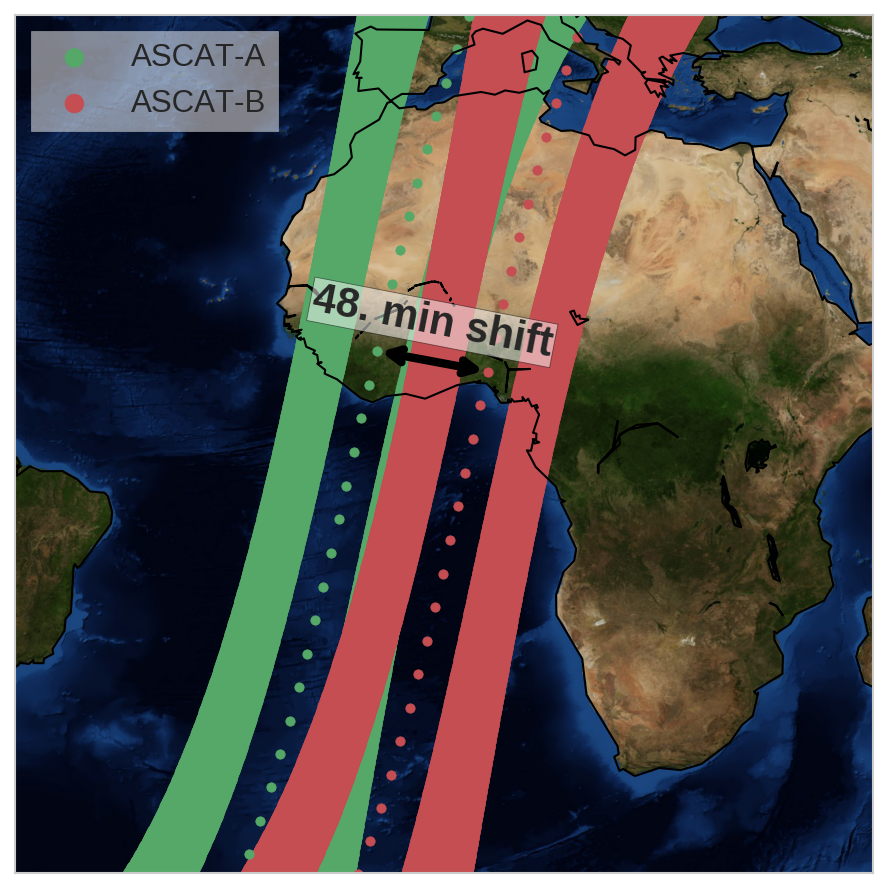
\includegraphics[width=0.85\textwidth]{./figures/ASCAT_AB_phasing.png}
\caption{Orbit Phasing ASCAT-A and ASCAT-B}
\end{figure}

\end{columns}

\end{frame}

\begin{frame}{Revisit time statistics}

\begin{figure}
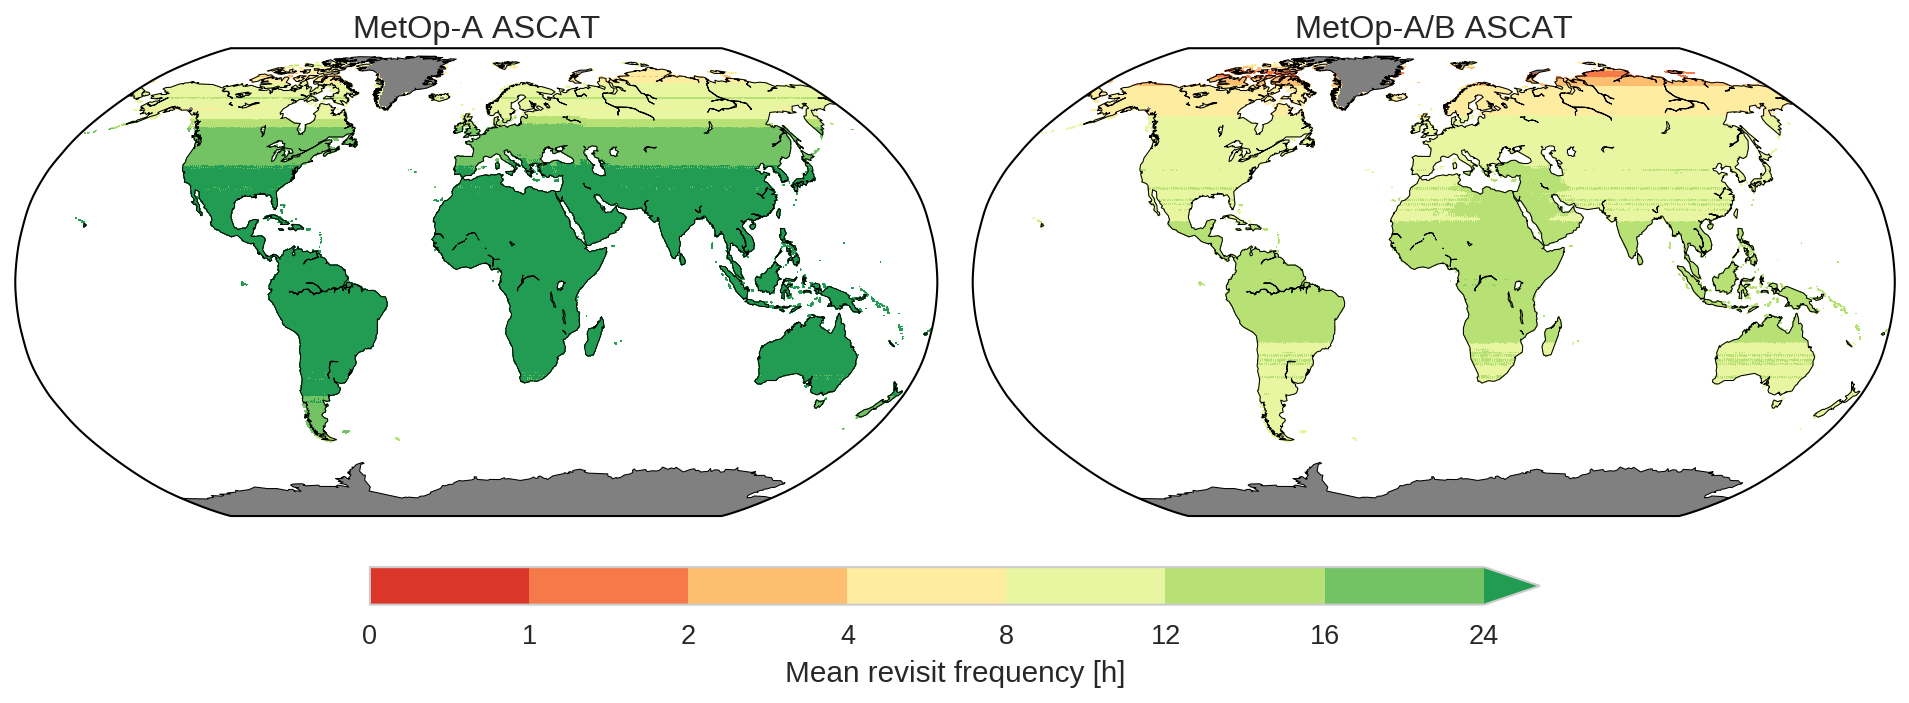
\includegraphics[width=0.85\textwidth]{./figures/revisit_freq_map_mean.png}
\end{figure}

\begin{figure}
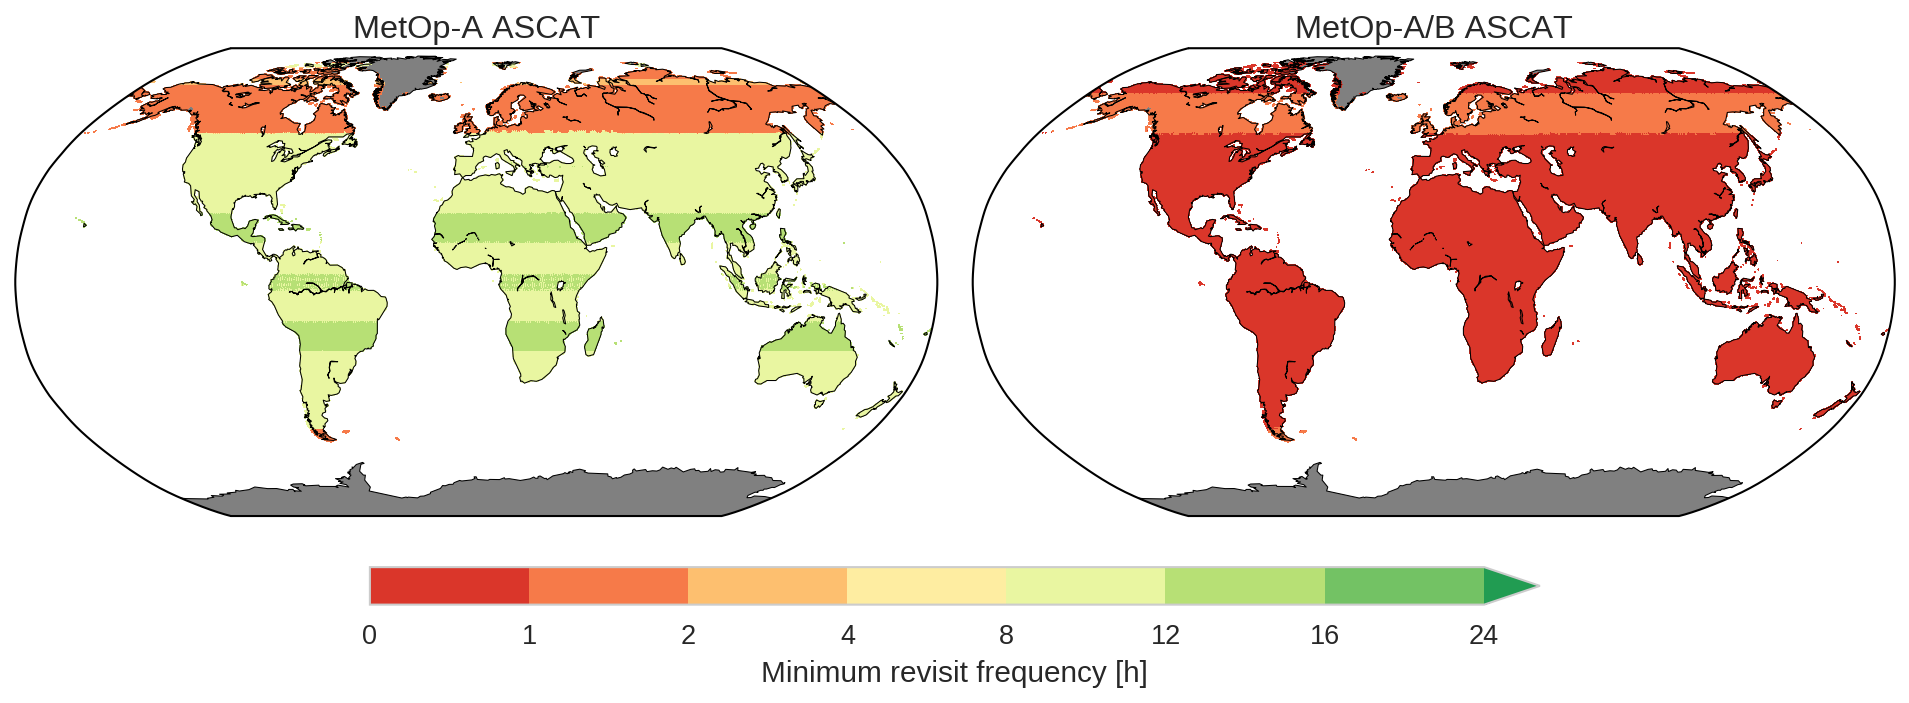
\includegraphics[width=0.85\textwidth]{./figures/revisit_freq_map_min.png}
\end{figure}

\end{frame}

\begin{frame}{Soil Moisture Processing @ TU Wien}

\begin{figure}
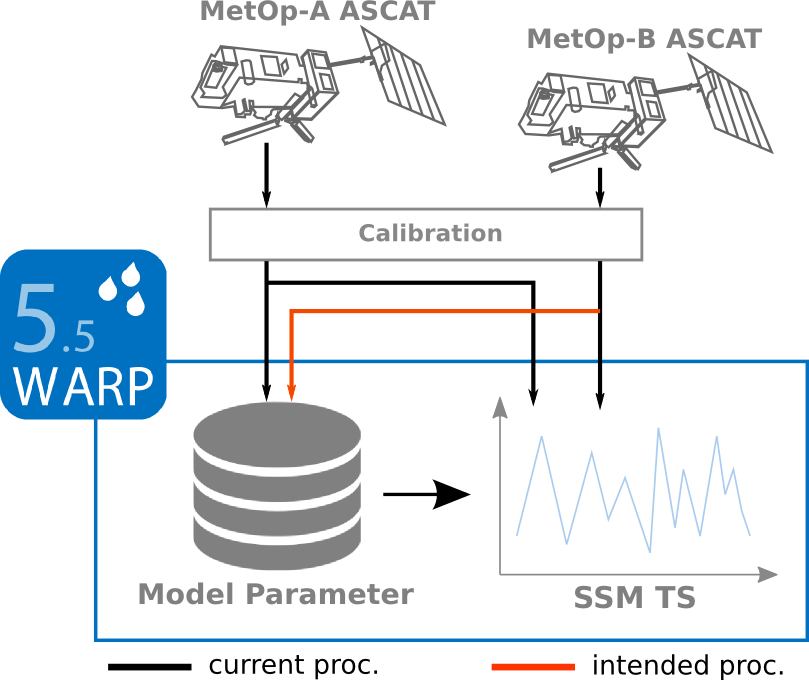
\includegraphics[width=0.65\textwidth]{./figures/warp_processing.png}
\end{figure}

\begin{center}
\textbf{optimal solution to use both sensors for MP.}

\newline

\textcolor{red}{\textbf{What do we have to consider in MP estimation?}}
\end{center}

\end{frame}

\begin{frame}{ASCAT-B Level 1b calibration status}

\begin{itemize}
\tightlist
\item
  Soil moisture retrieval requires long-term stability
\item
  Instrument monitoring over Rainforests

  \begin{itemize}
  \tightlist
  \item
    Amazon, Congo and Indonesia Rainforest
  \end{itemize}
\item
  Gamma model vs.~TU Wien model (2nd order polynomial)
\end{itemize}

\begin{columns}

\column{0.4\textwidth}

\begin{figure}
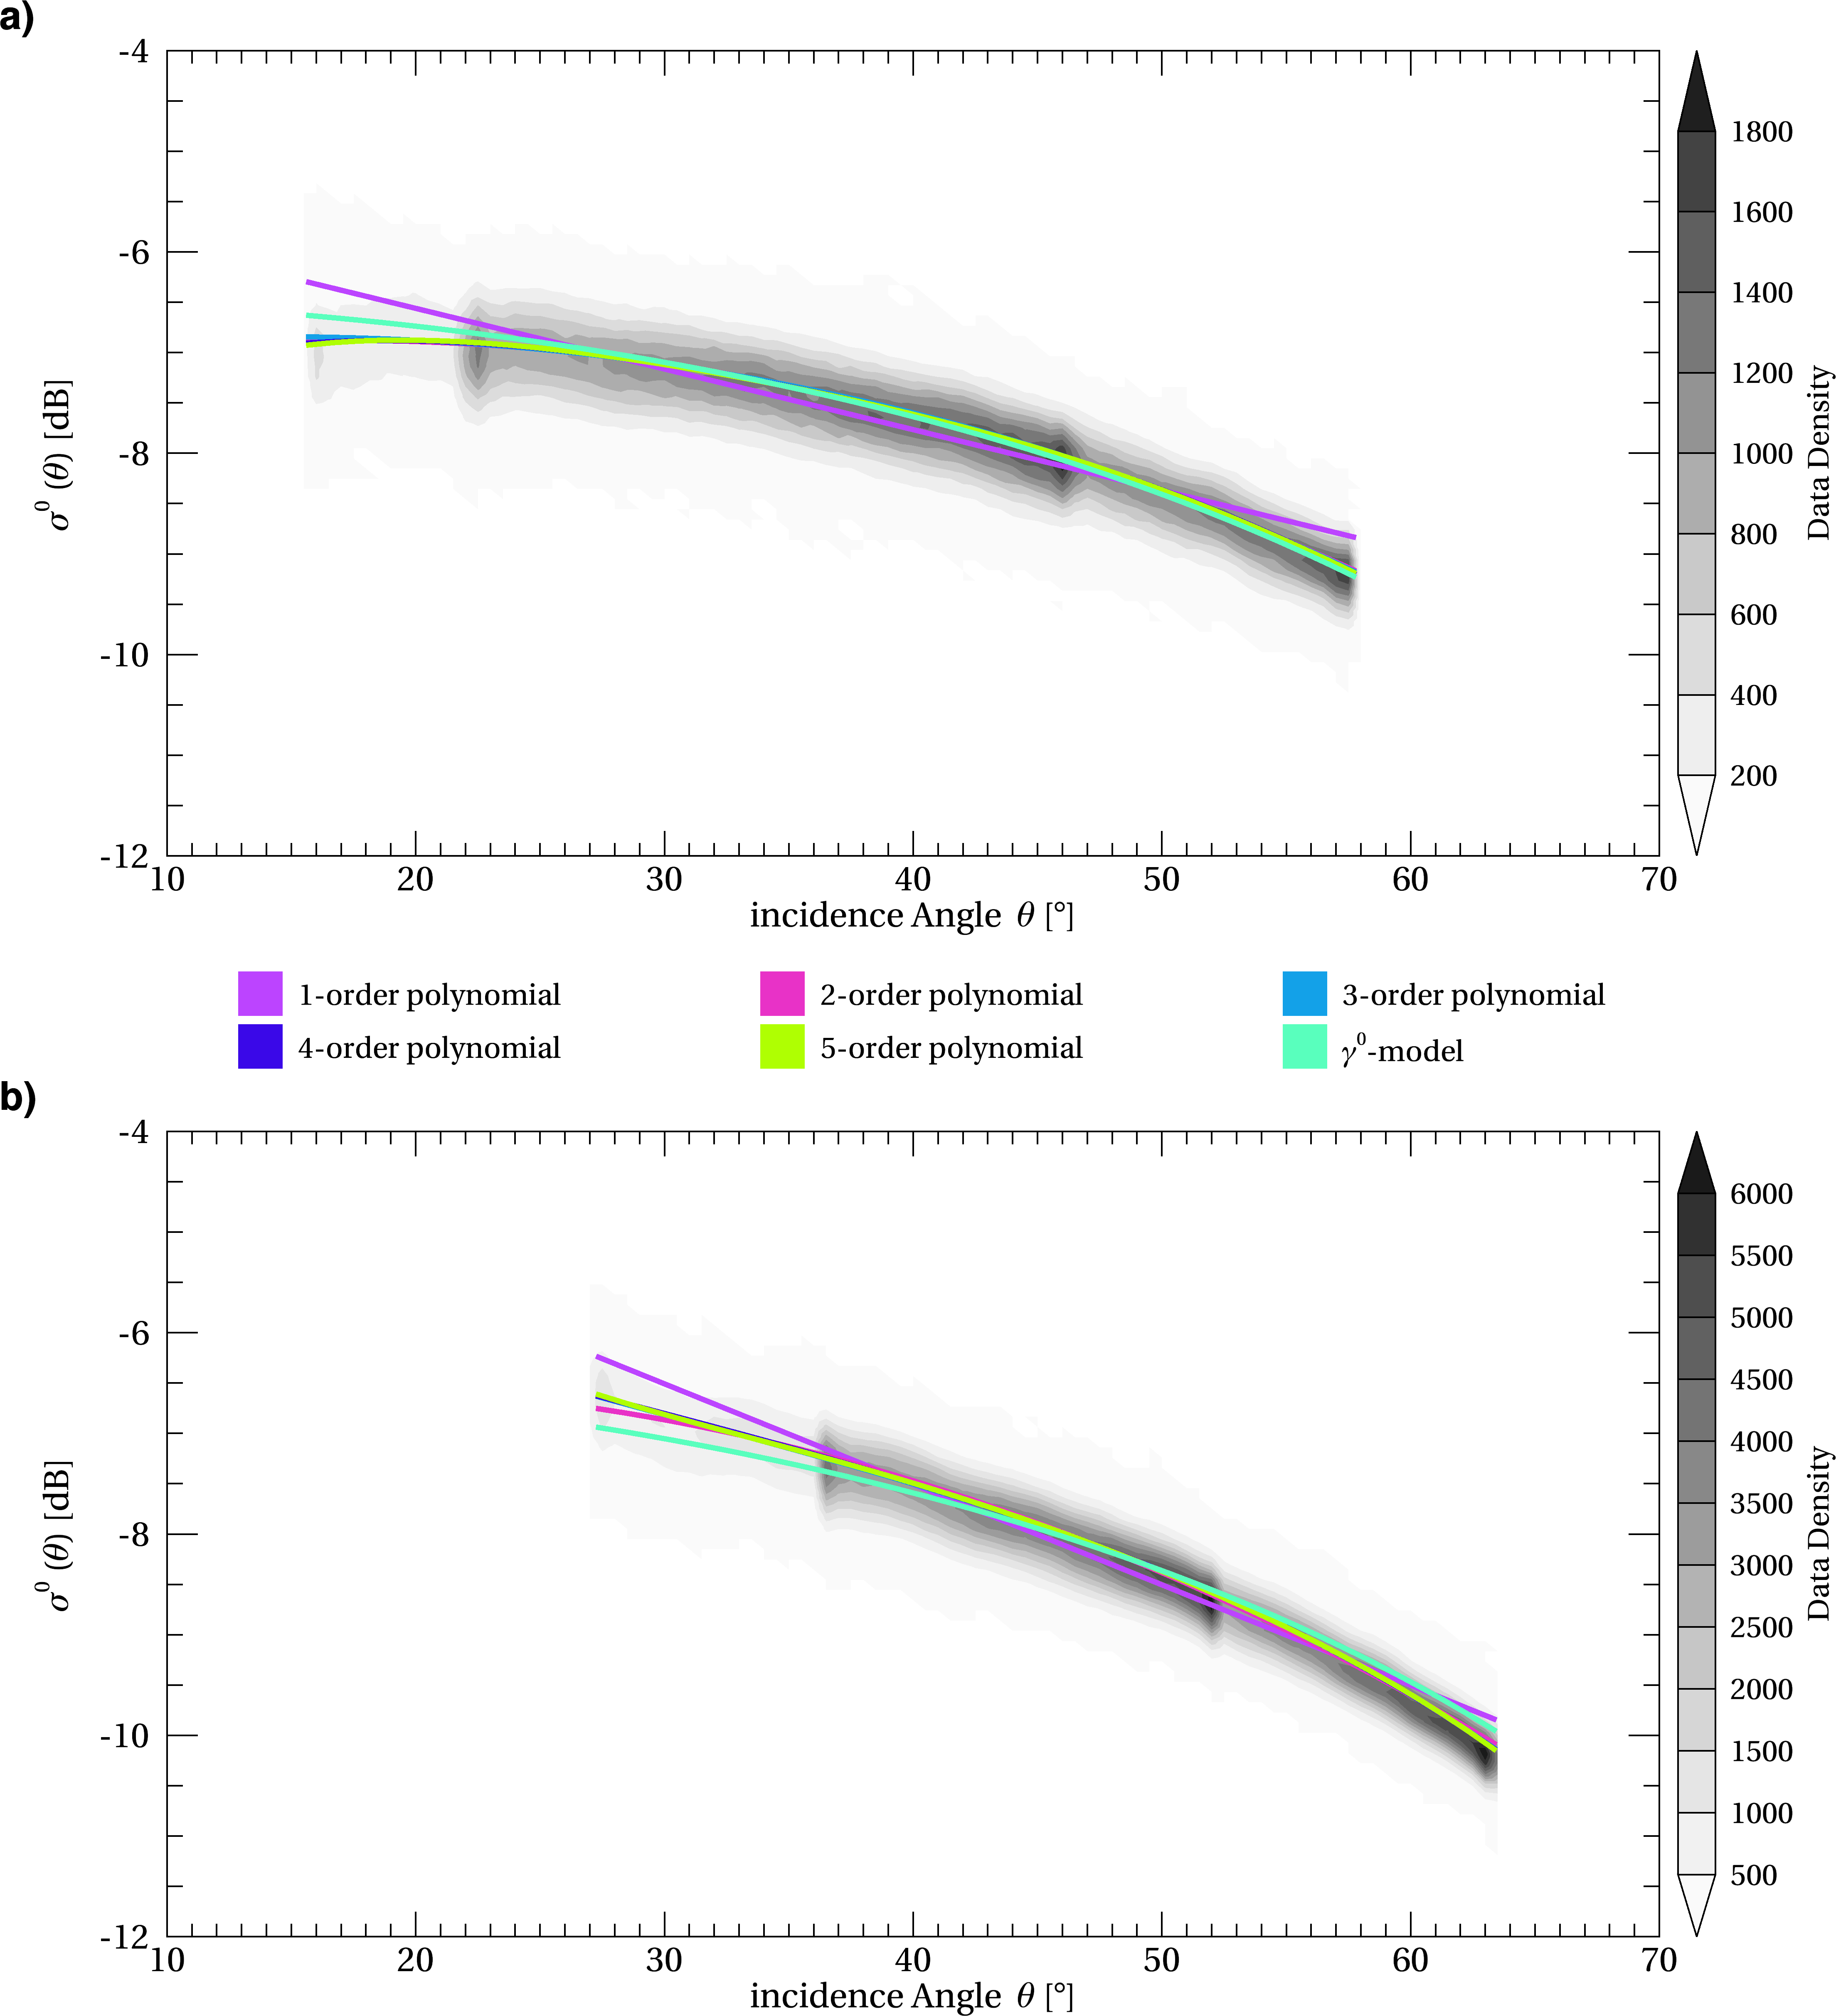
\includegraphics[width=.99\textwidth]{./figures/Backscatter_Models.png}
\caption{a) ERS-2 ESCAT b) MetOp-A ASCAT}
\end{figure}

\column{0.6\textwidth}

\begin{figure}
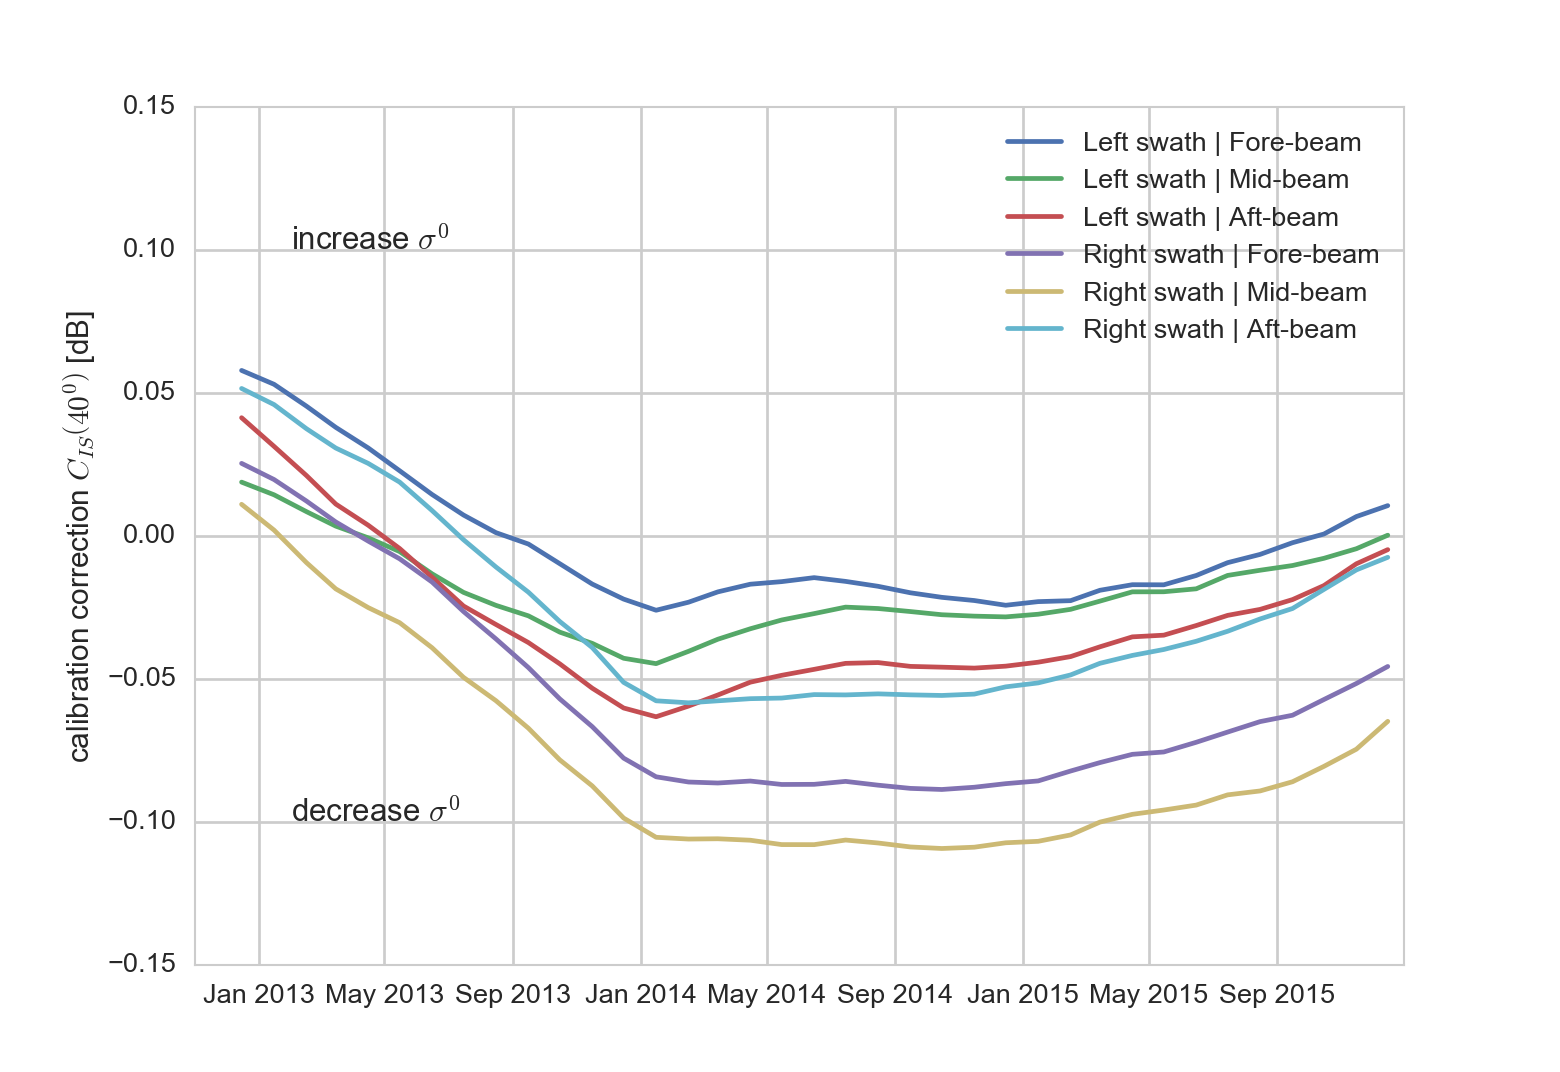
\includegraphics[width=.99\textwidth]{./figures/metop_b_ascat_calibration.png}
\end{figure}

\end{columns}

\end{frame}

\begin{frame}{Calibration induced SM bias}

\begin{center}
\textbf{Level 1 calibration bias of 0.1 dB between ASCAT-A and ASCAT-B}
\end{center}

\begin{figure}
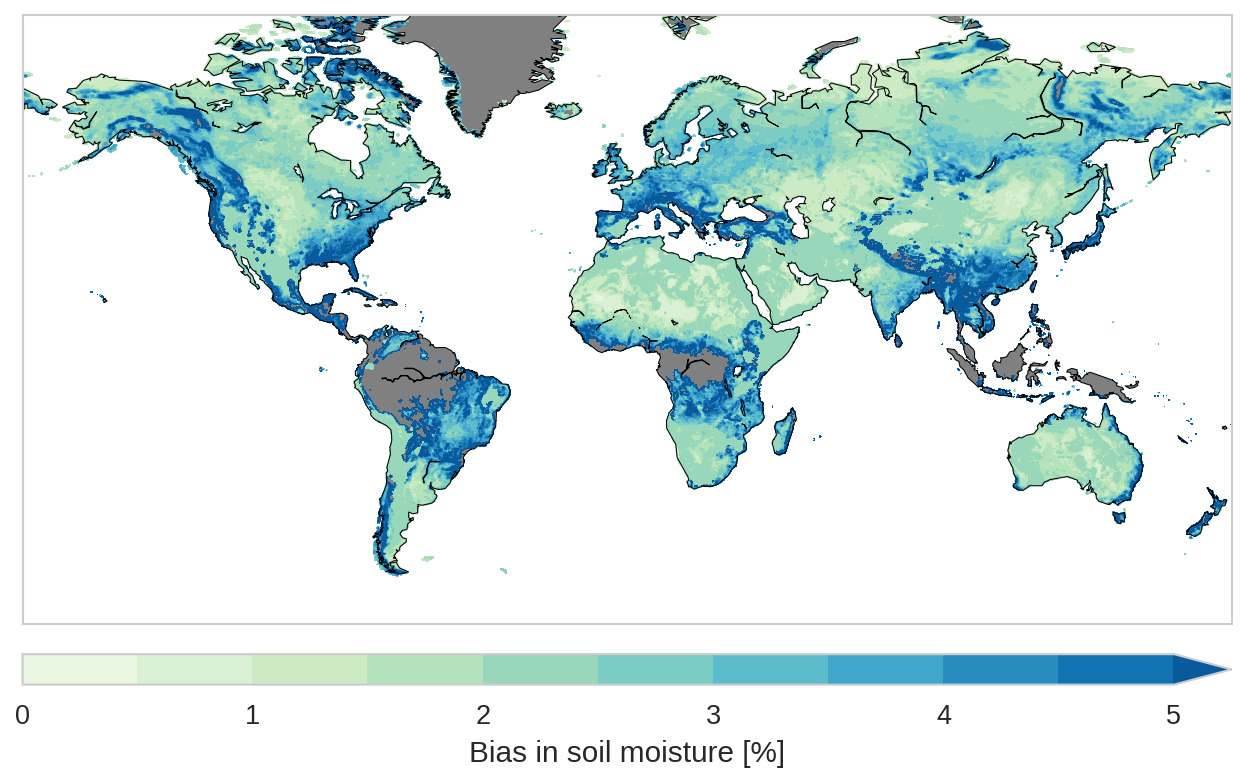
\includegraphics[width=.9\textwidth]{./figures/metop_b_ssm_cal_bias.png}
\end{figure}

\end{frame}

\begin{frame}{Soil moisture model parameter estimation}

\begin{columns}

\column{0.4\textwidth}

\begin{itemize}
\tightlist
\item
  TU Wien SM retrieval is a physically motivated semi-empirical change
  detection method
\item
  Calibration of model parameters (MP) required to separate different
  backscatter contributions

  \begin{itemize}
  \tightlist
  \item
    MP estimation is based on \enquote{inter-annual} time series
    analysis
  \end{itemize}
\item
  Comparison of MP derived from

  \begin{itemize}
  \tightlist
  \item
    ASCAT-A (2007 - 2015)
  \item
    ASCAT-B (2013 - 2015)
  \item
    ASCAT-AB (2007- 2015)
  \end{itemize}
\end{itemize}

\column{0.6\textwidth}

\begin{figure}
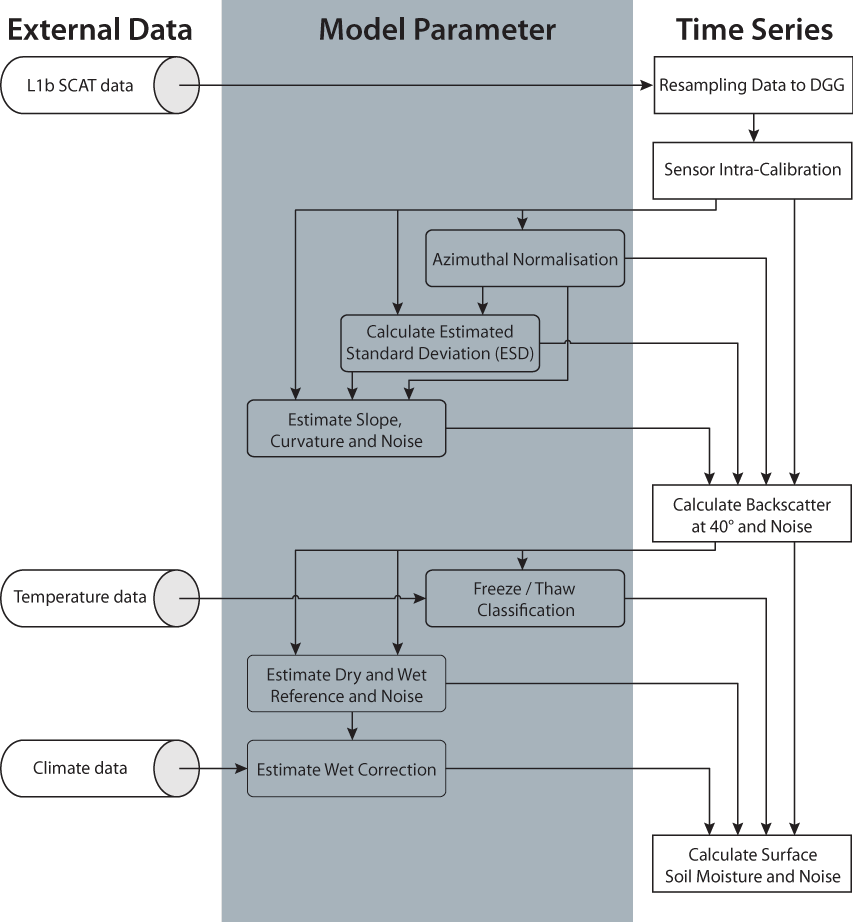
\includegraphics[width=.75\textwidth]{./figures/warp.png}
\end{figure}

\end{columns}

\end{frame}

\begin{frame}{Estimated Standard Deviation (ESD)}

\begin{itemize}
\tightlist
\item
  Backscatter noise estimate for SM error model
\item
  Estimated using: \(\delta = \sigma^{0}_{fore} - \sigma^{0}_{aft}\)
\end{itemize}

\[ESD\left(\sigma^{\circ}\right) = \frac{SD\left[\delta\right]}{\sqrt{2}}\]

\vspace{.2cm}

\begin{figure}
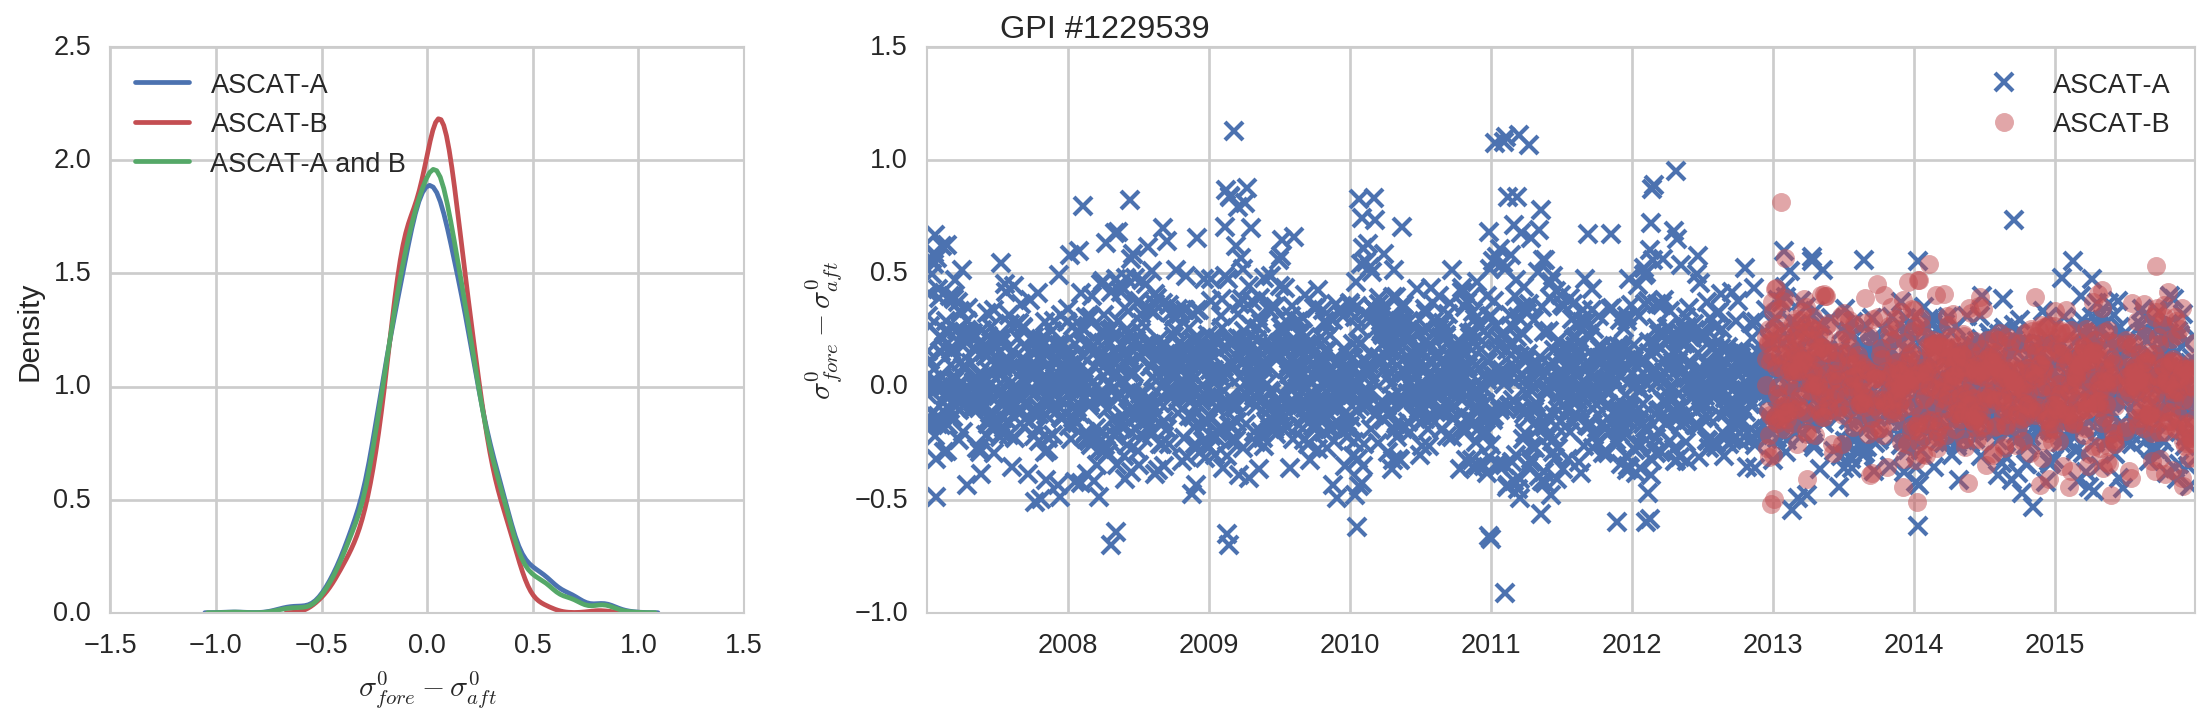
\includegraphics[width=.9\textwidth]{./figures/esd_difference_GPI1229539.png}
\end{figure}

\end{frame}

\begin{frame}{Azimuth normalisation coefficients}

\begin{itemize}
\tightlist
\item
  Account for azimuthal anisotropy effects in backscatter
\item
  12 azimuth observation configurations (3 x beams, 2 x swath, 2 x
  overpasses)
\item
  Difference to statistically expected backscatter

  \begin{itemize}
  \tightlist
  \item
    2nd order polynomial
  \end{itemize}
\end{itemize}

\begin{figure}
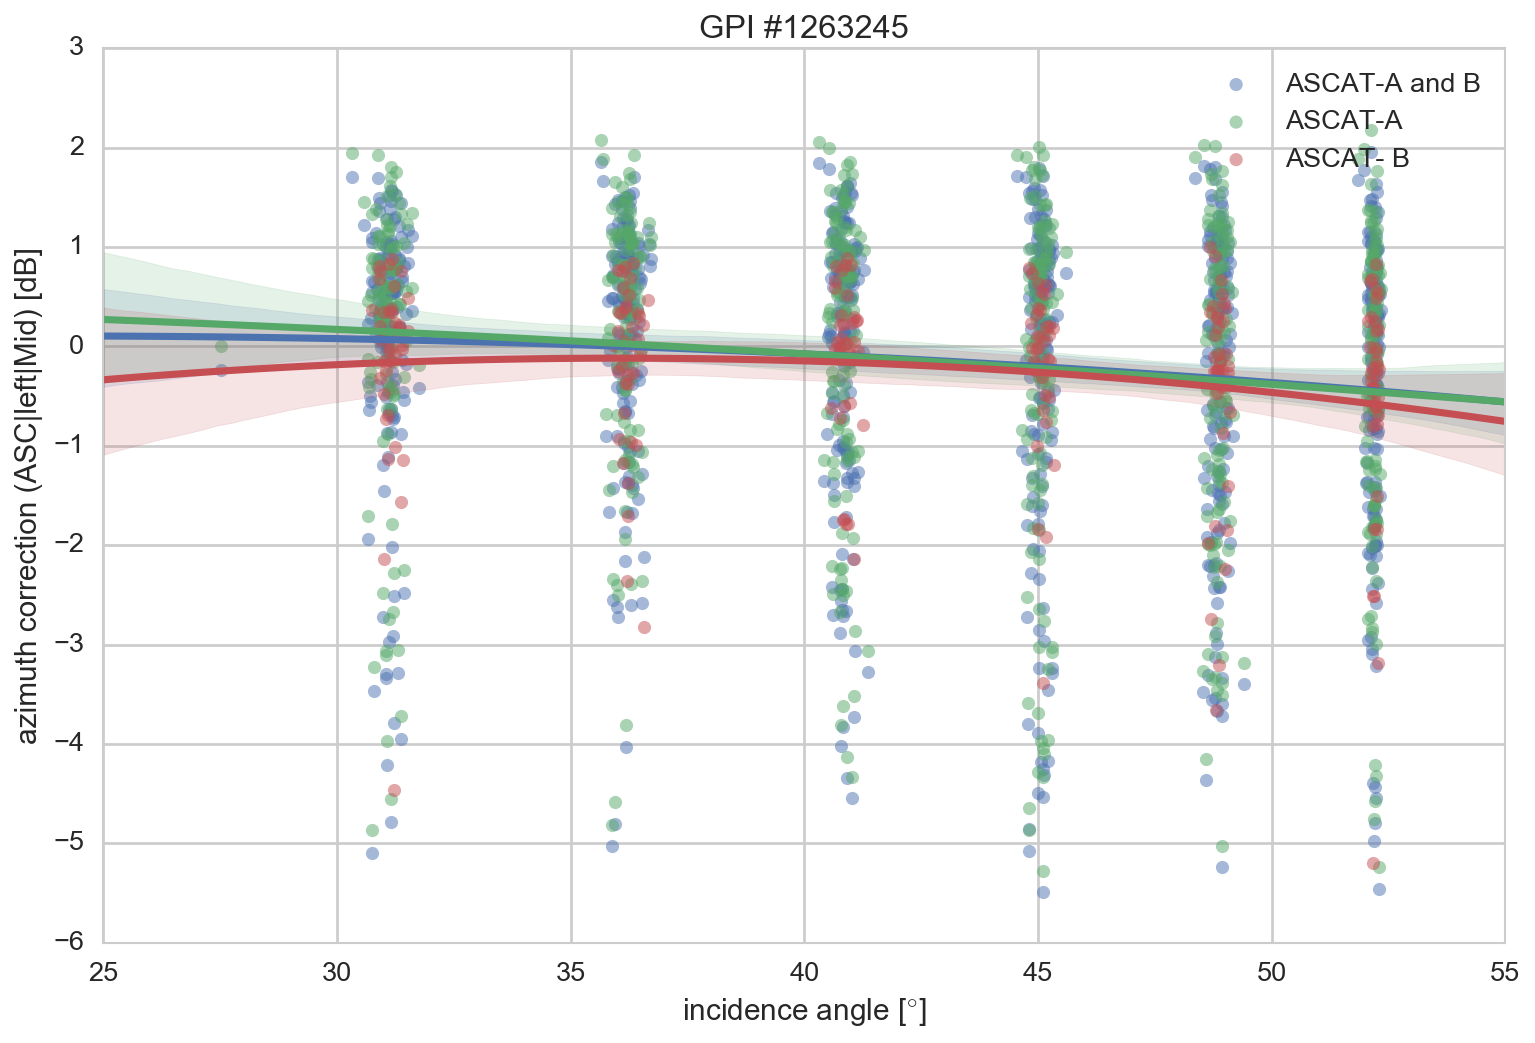
\includegraphics[width=.6\textwidth]{./figures/azimuth_difference_GPI1263245.png}
\end{figure}

\end{frame}

\begin{frame}{Incidence angle normalisation (Slope)}

\begin{itemize}
\tightlist
\item
  Inc. angle behaviour modelled via 2nd order Taylor polynomial
\item
  Slope \(\sigma^{\prime}\) = first derivative of inc. angle behaviour
\end{itemize}

\[\sigma^{\circ}\left(\theta,t\right) =
\sigma^{\circ}\left(\theta_{ref}, t\right) +
\sigma^{\prime}\left(\theta_{ref},
t\right)\left(\theta-\theta_{ref}\right) +
\frac{1}{2}\cdot\sigma^{\prime\prime}\left(\theta_{ref},
t\right)\left(\theta-\theta_{ref}\right)^{2}\]

\begin{figure}
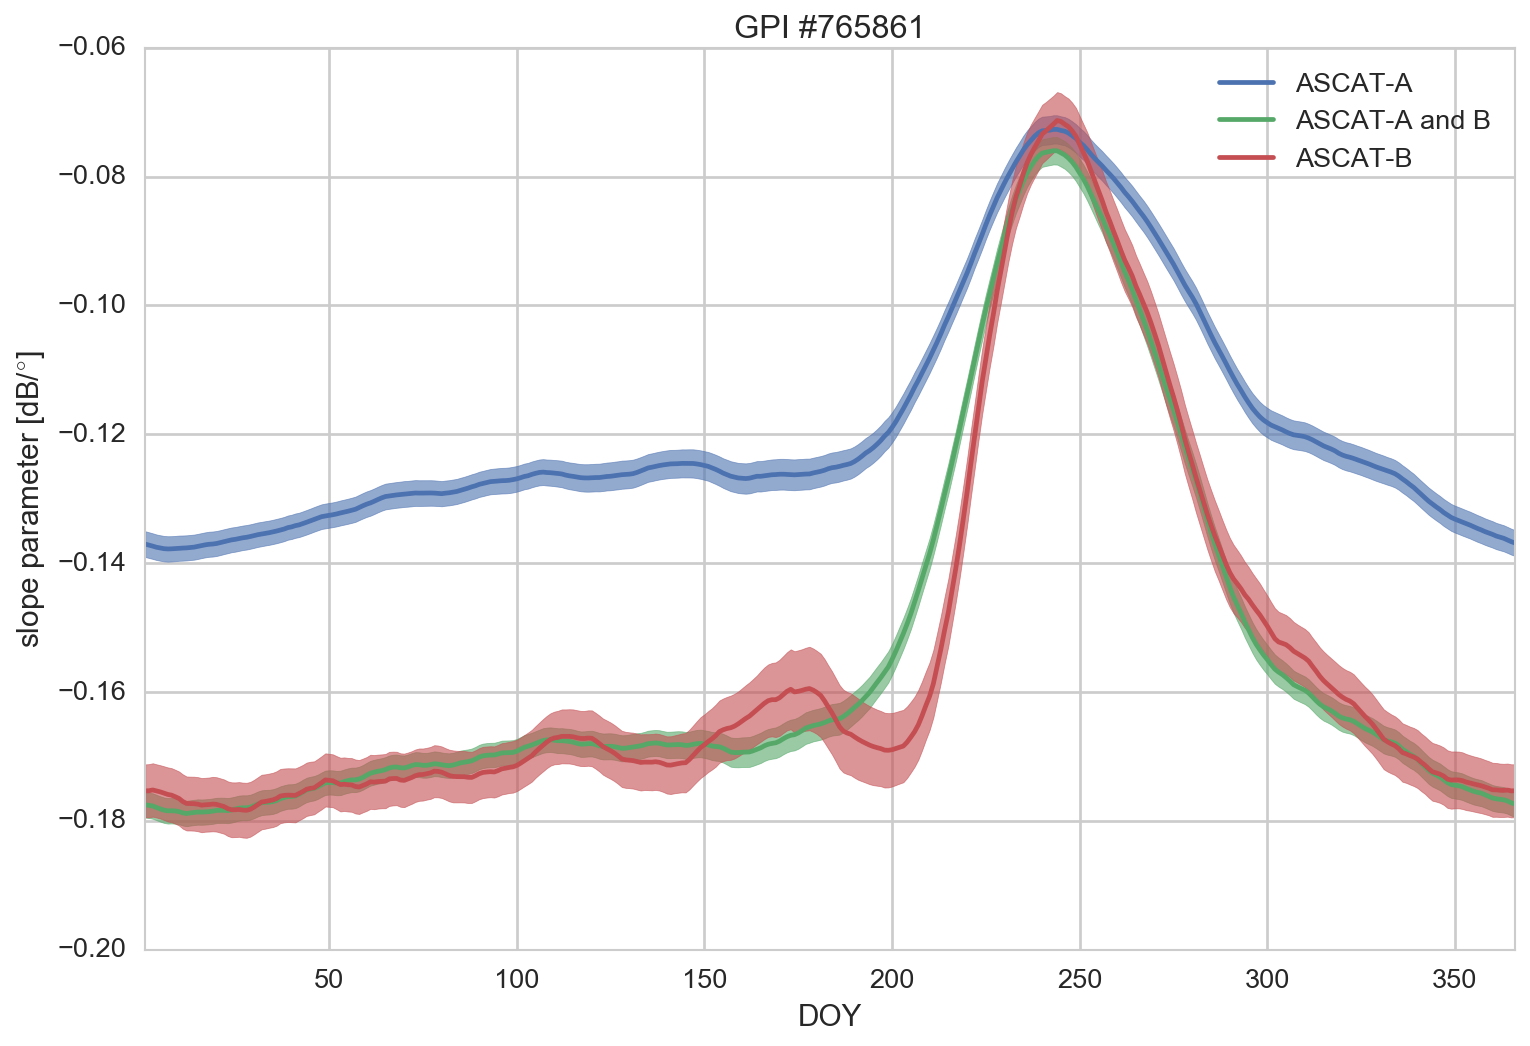
\includegraphics[width=.8\textwidth]{./figures/slope_difference_GPI765861.png}
\end{figure}

\end{frame}

\begin{frame}{Daily Slope estimation}

\begin{itemize}
\tightlist
\item
  Make use of LLR for lope estimation over time

  \begin{itemize}
  \tightlist
  \item
    critical parameter \(\Rightarrow\) time window length
  \end{itemize}
\item
  Bias in Slope due to bias in azimuth norm.

  \begin{itemize}
  \tightlist
  \item
    identical temporal behaviour of ASCAT-A / ASCAT-B
  \end{itemize}
\end{itemize}

\begin{figure}
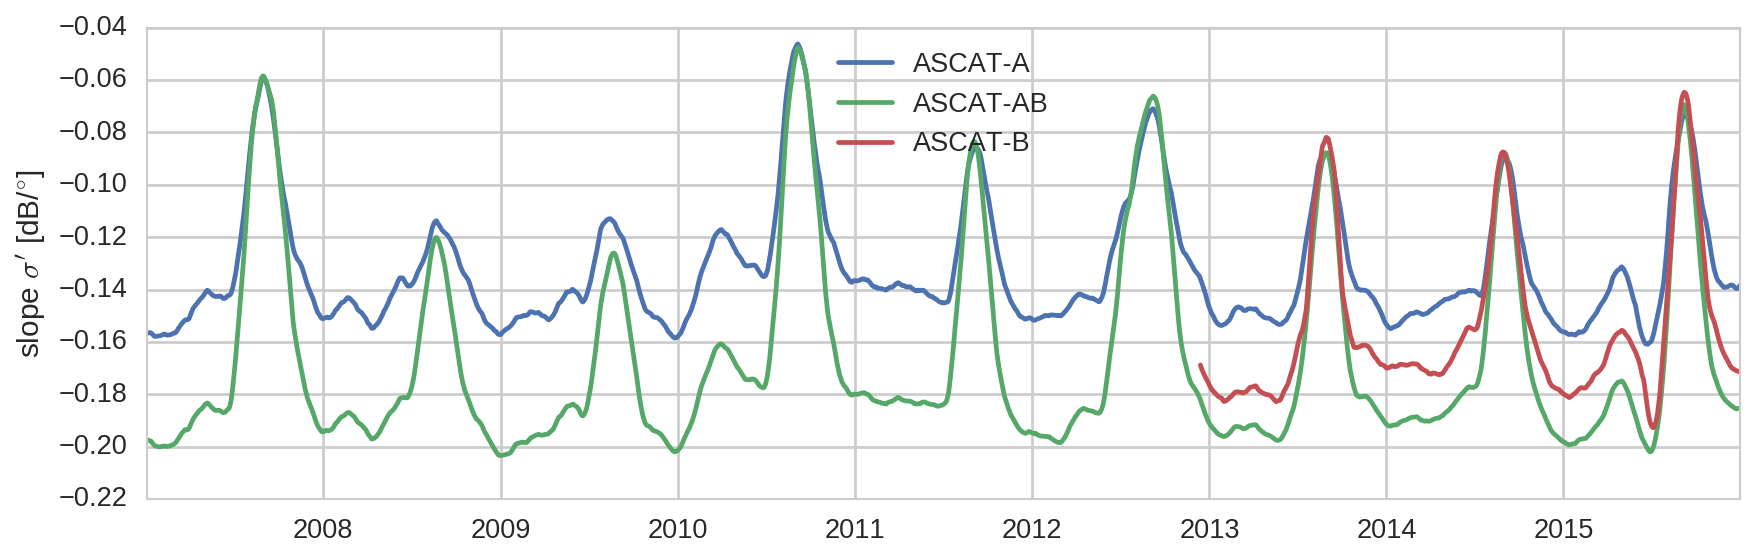
\includegraphics[width=.75\textwidth]{./figures/daily_slope_estimates_GPI765861.png}
\end{figure}

\end{frame}

\begin{frame}{Dry/Wet reference}

\begin{itemize}
\tightlist
\item
  Representing the driest and wettest observed soil moisture condition.
\end{itemize}

\begin{center}
$m_{s}\left(t\right) = \frac{\sigma^{\circ}\left(\theta_{ref},t\right) -
\sigma^{\circ}_{dry}\left(\theta_{ref},t\right)}{\sigma^{\circ}_{wet}\left(\theta_{ref},t\right) -
\sigma^{\circ}_{dry}\left(\theta_{ref},t\right)} \qquad
[\text{degree of saturation}]$
\end{center}

\begin{figure}
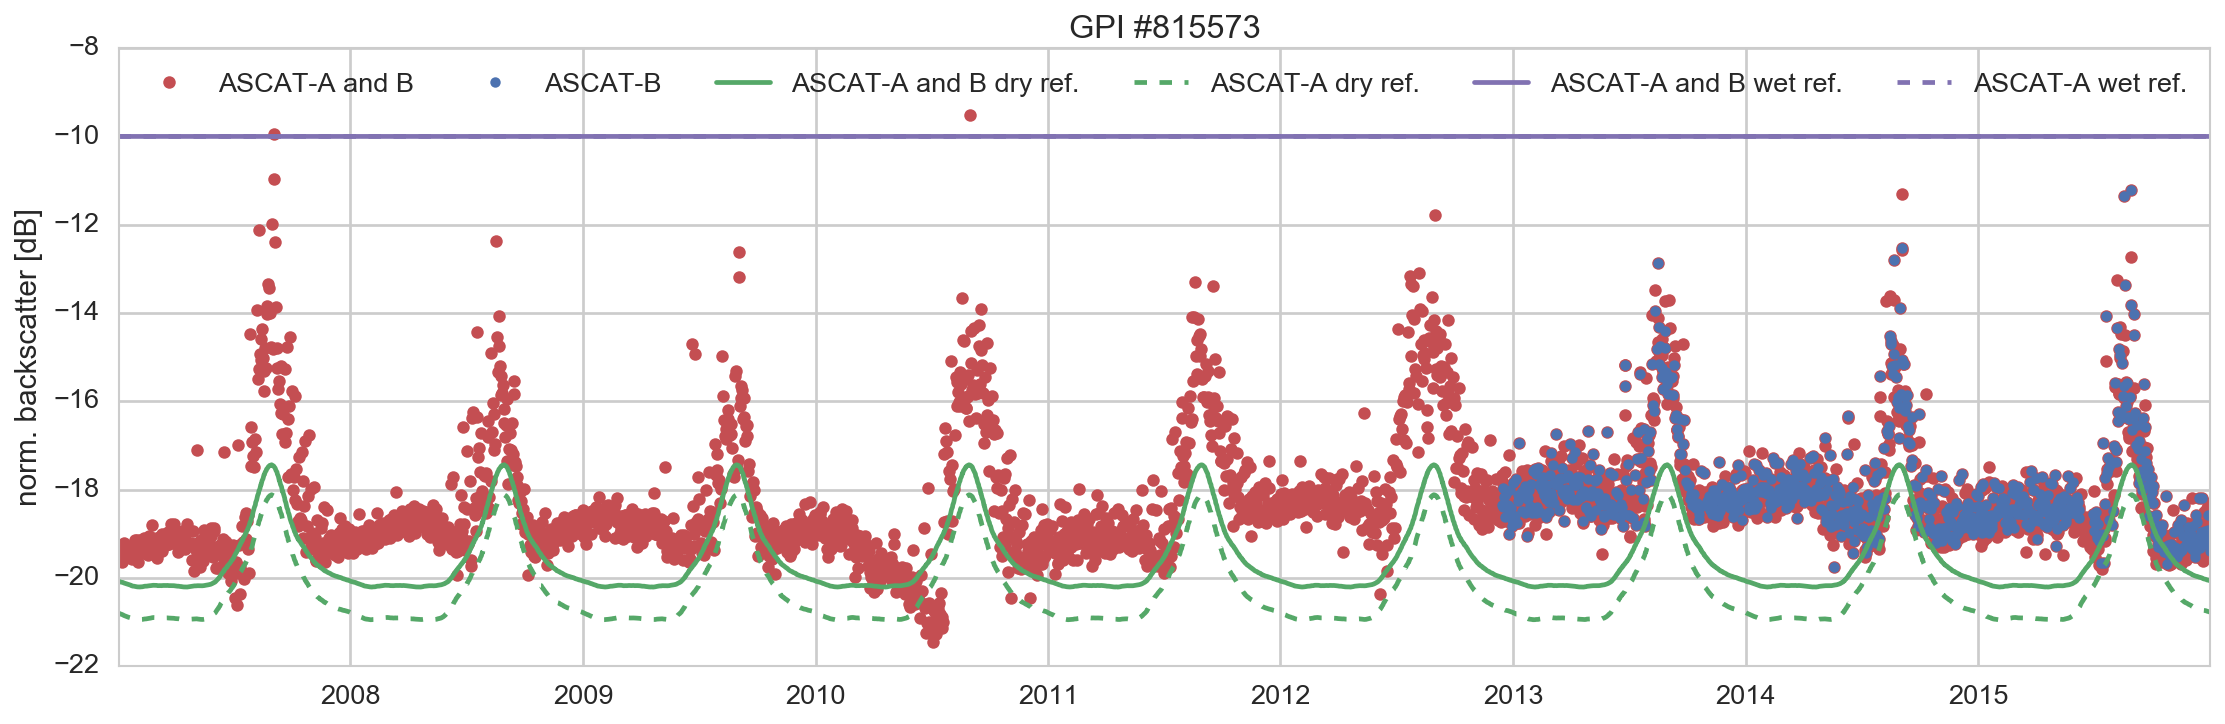
\includegraphics[width=.8\textwidth]{./figures/norm_sigma_dry_wet_GPI815573.png}
\end{figure}

\end{frame}

\begin{frame}{Validation with respect to in-situ soil moisture}

\begin{itemize}
\tightlist
\item
  What is the impact on the final SM retrievals?

  \begin{itemize}
  \tightlist
  \item
    Validation of three ASCAT SM products
  \end{itemize}
\item
  ISMN in-situ data

  \begin{itemize}
  \tightlist
  \item
    32 networks with 789 stations in total
  \item
    Sensor depths: 0 -- 0.10m
  \end{itemize}
\item
  Data Manipulation

  \begin{itemize}
  \tightlist
  \item
    Masking for snow, soil temperature, Freeze/Thaw state
  \item
    Min / Max scaling of ASCAT to in-situ soil moisture
  \item
    Temporal collocation with 8h time window
  \end{itemize}
\end{itemize}

\end{frame}

\begin{frame}{In-situ validation results per network}

\begin{figure}
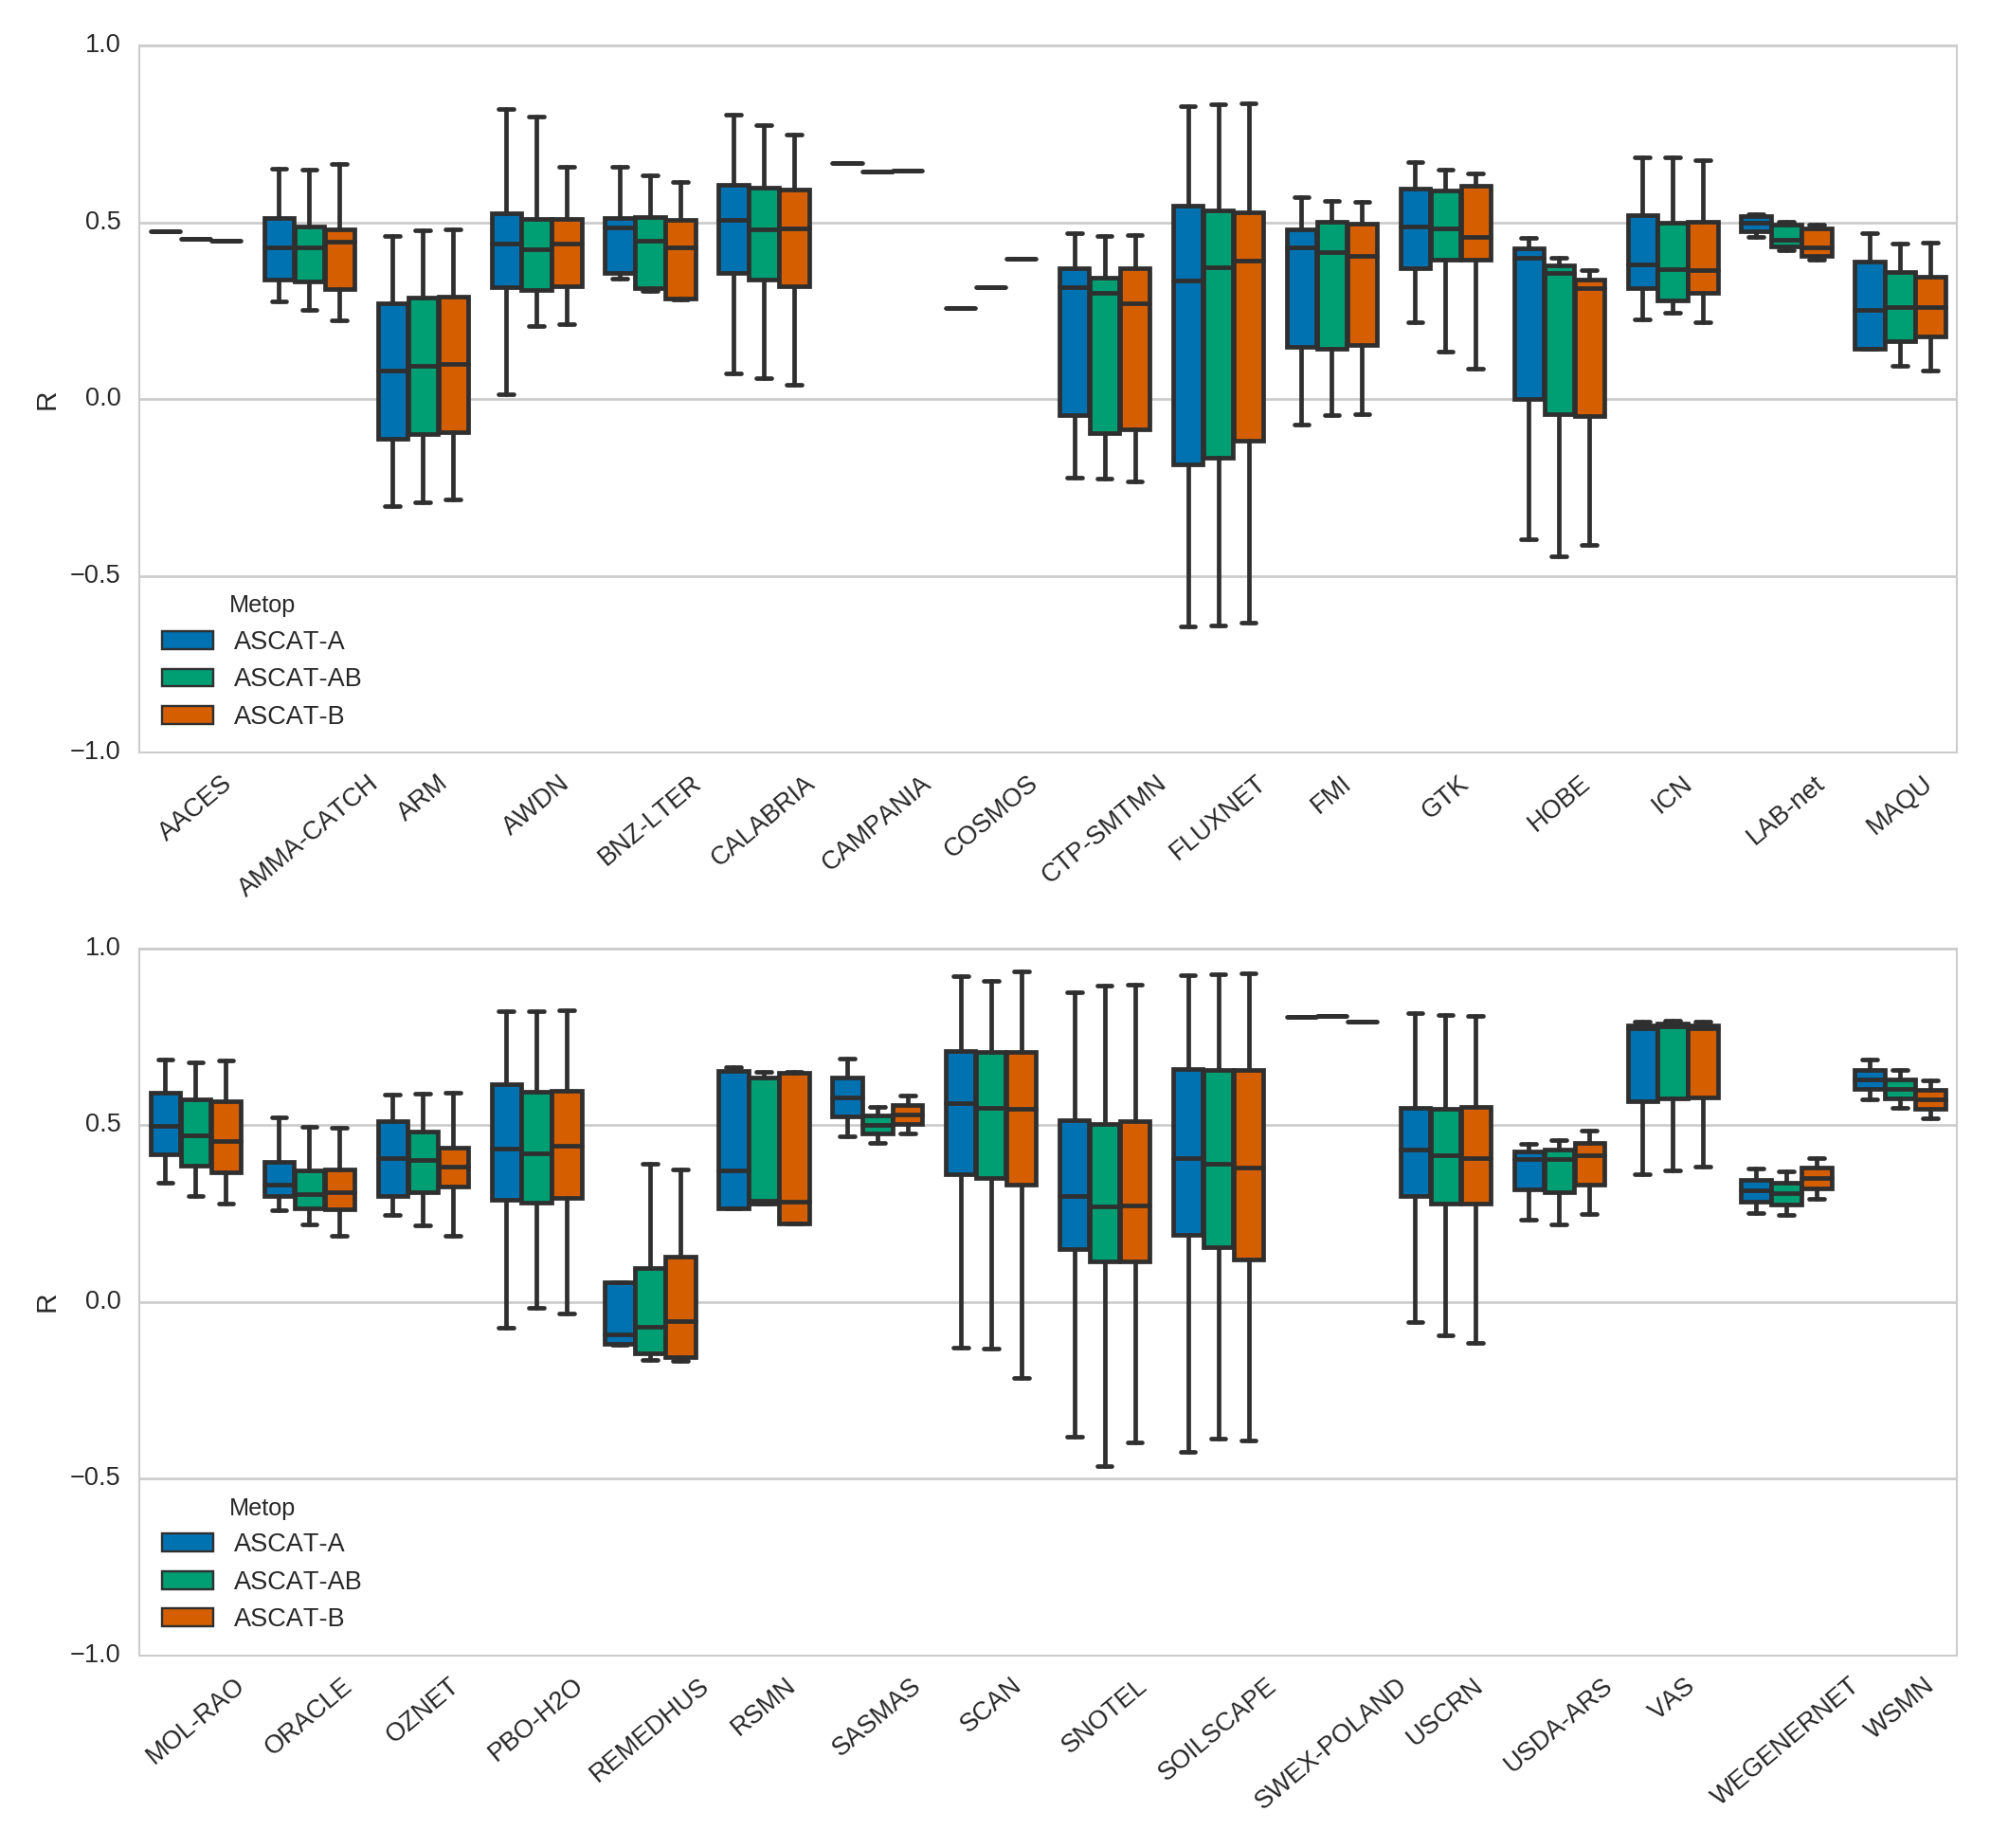
\includegraphics[height=0.8\textheight,keepaspectratio]{./figures/boxplot_ISMNnetwork_ASCAT.png}
\end{figure}

\end{frame}

\begin{frame}{In-situ validation results global summary}

\begin{figure}
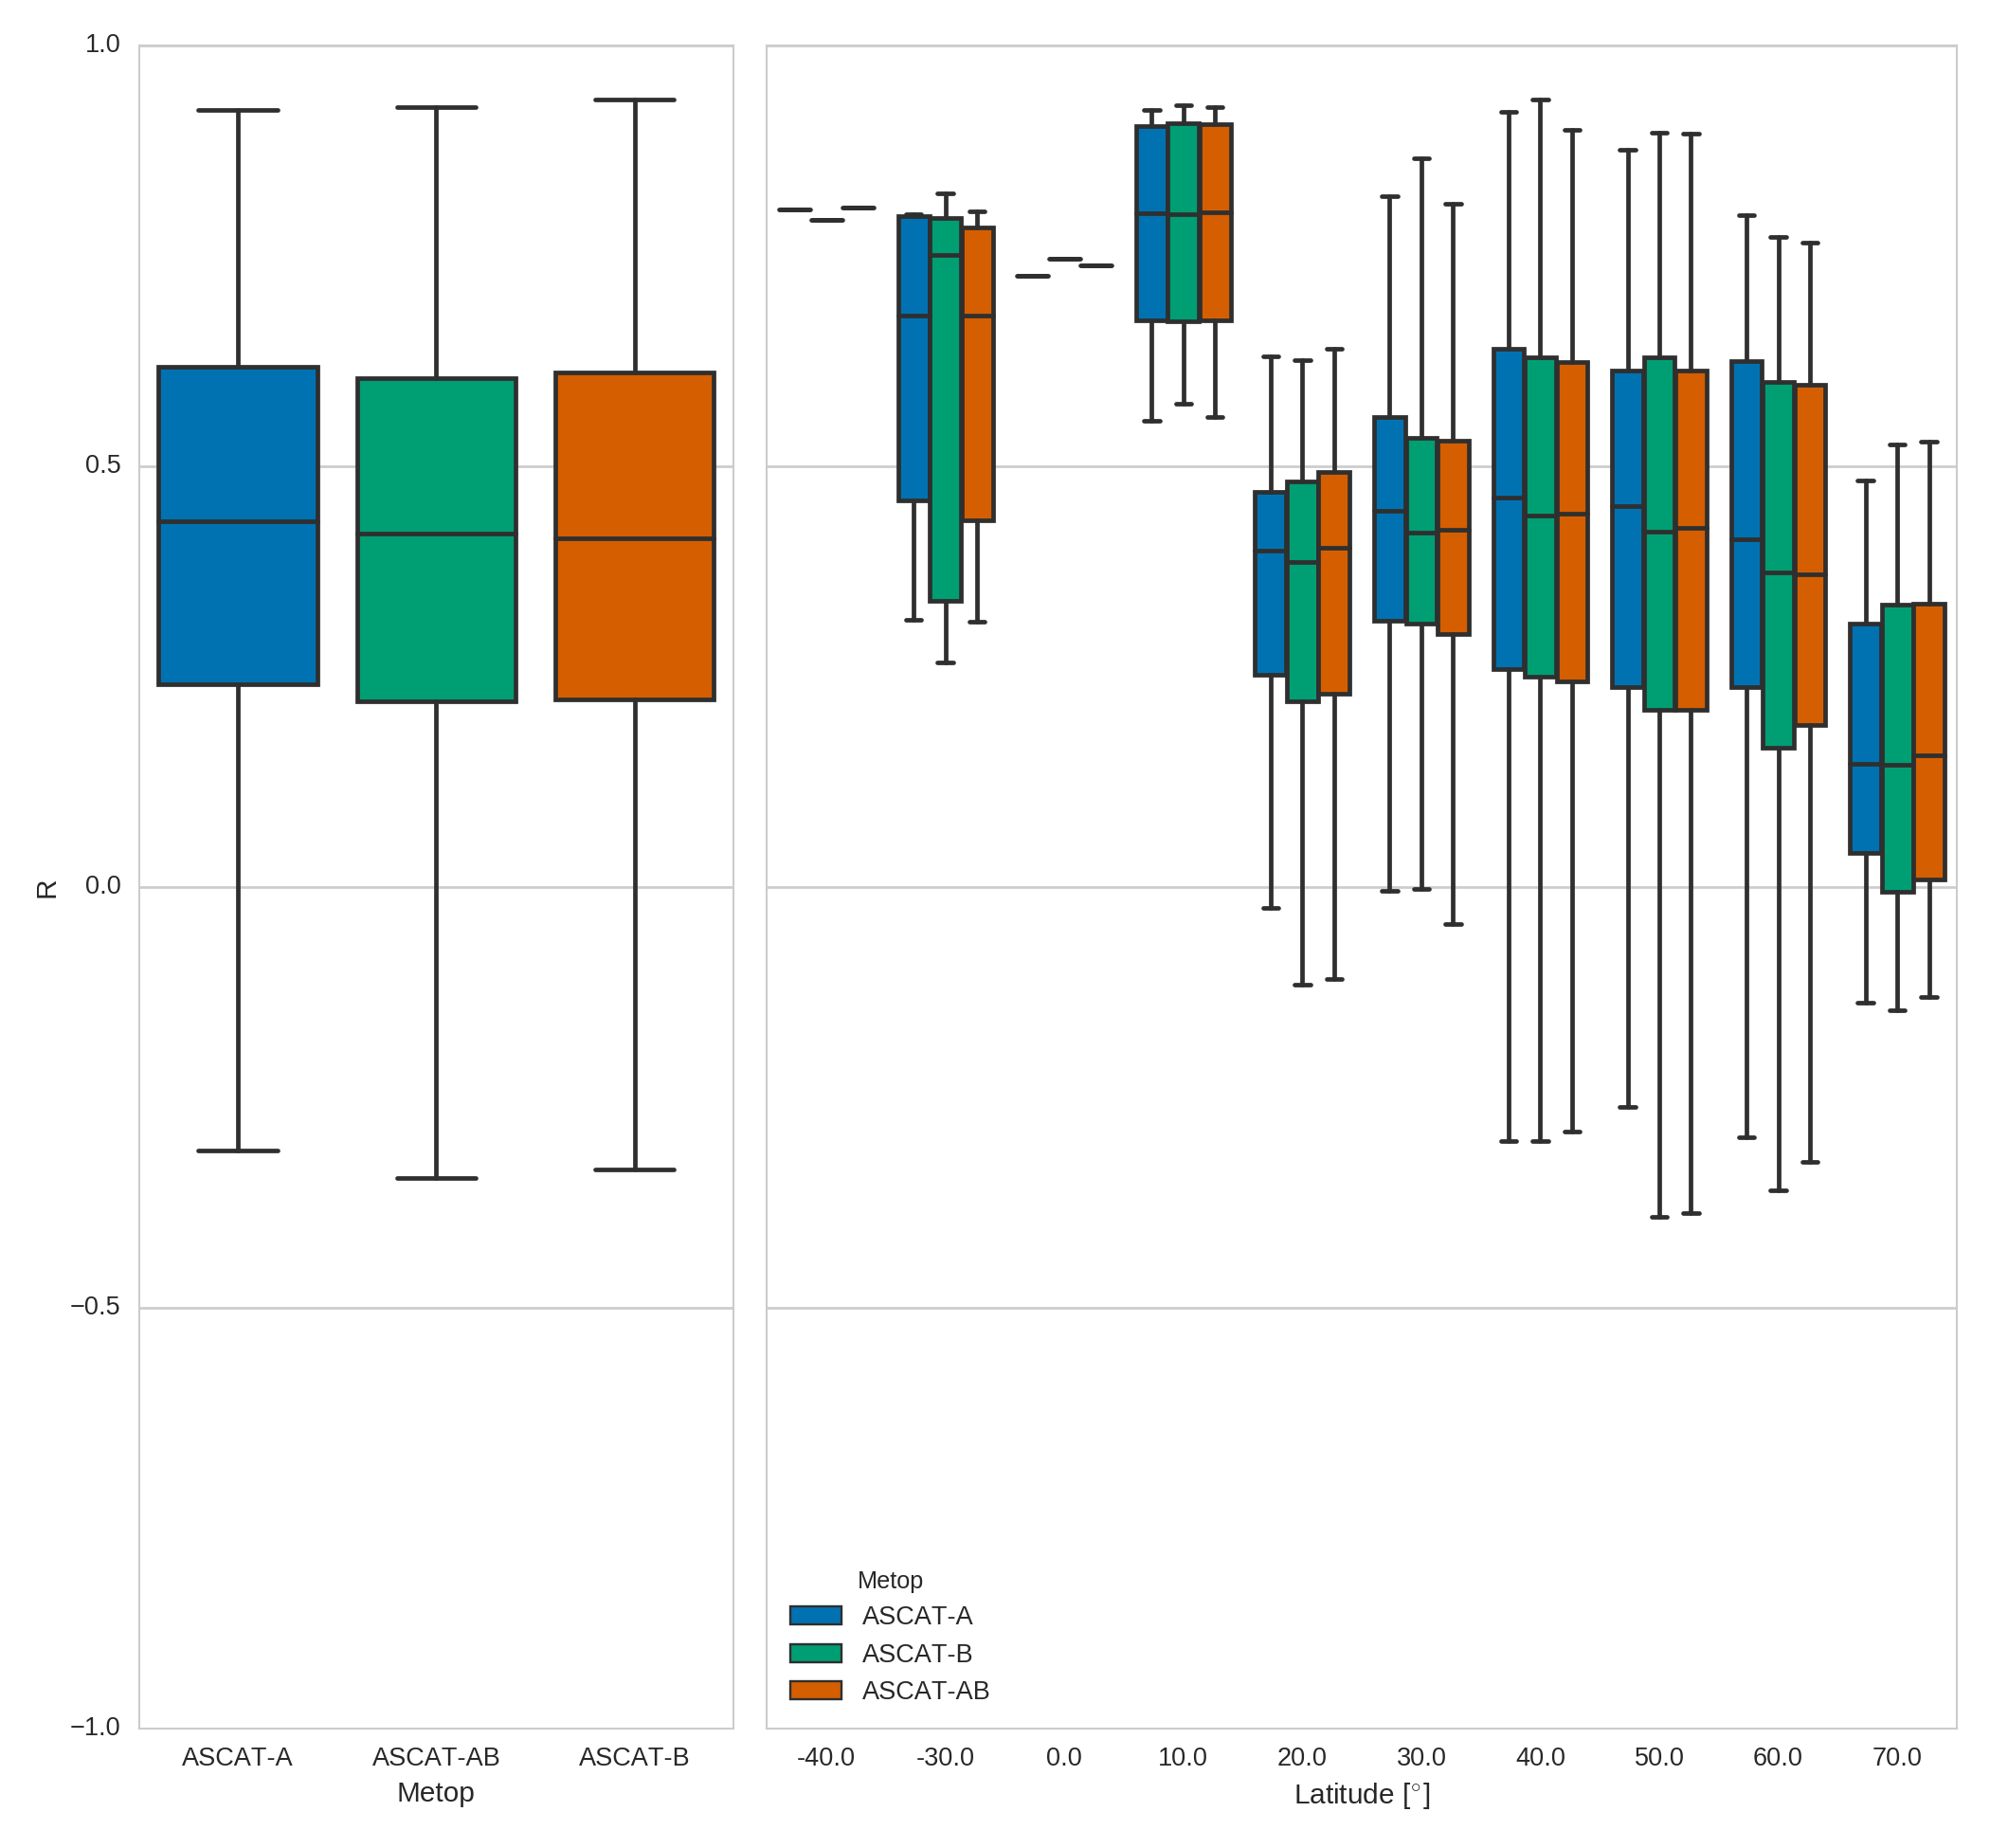
\includegraphics[height=0.8\textheight,keepaspectratio]{./figures/boxplot_ISMN_ASCAT_all_latitude.png}
\end{figure}

\end{frame}

\begin{frame}{Soil Moisture Validation ERA-interim}

\begin{figure}
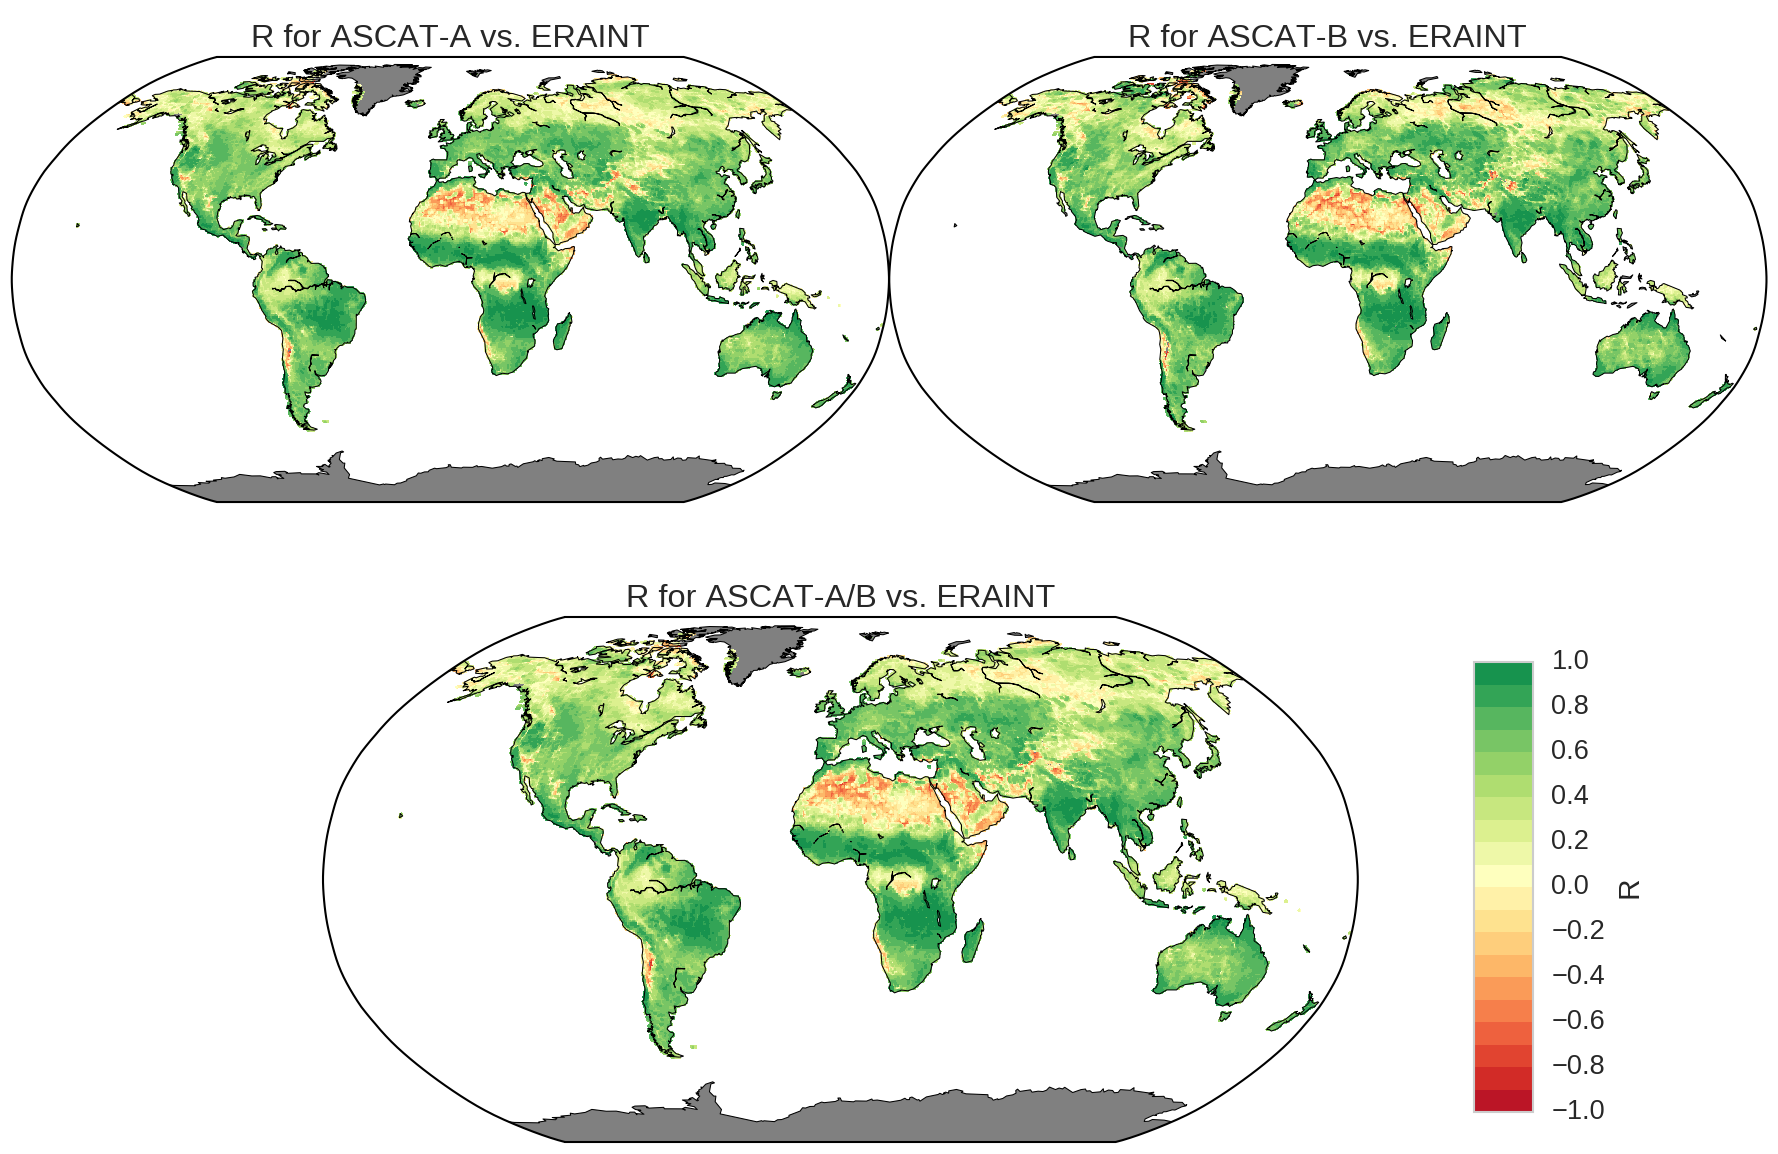
\includegraphics[width=.9\textwidth]{./figures/ASCAT_ERAINT_maps_crop.png}
\end{figure}\begin{center}
\textbf{Negative impact over desert regions.}
\end{center}

\end{frame}

\begin{frame}{Conclusion}

\begin{itemize}
\item
  Tandem scenario of ASCAT result in a mean revisit time of less than 16
  h globally.
\item
  Inter-calibration of ASCAT-A and ASCAT-B critical for SM retrieval

  \begin{itemize}
  \tightlist
  \item
    A 0.1 dB difference will introduce a bias of about 3\% in soil
    moisture
  \end{itemize}
\item
  Impact of tandem phase scenario on model parameter estimation

  \begin{itemize}
  \tightlist
  \item
    Good agreement with latest MPs in general
  \item
    Sensitivity of model parameters are different
  \item
    Account for correlations in ASCAT-A/B, by applying a weighting in
    the MP estimation
  \end{itemize}
\item
  In-situ validation indicates neutral impact
\item
  Validation against ERA-interim

  \begin{itemize}
  \tightlist
  \item
    Overall neutral impact
  \item
    Desert regions are exceptions
  \end{itemize}
\end{itemize}

\end{frame}





\end{document}
